\section{Where We Left Off}


\begin{frame}{Unfinished Business from Lecture 10}
    Hald cement data, all four regressors: $R^2=0.982$ and the overall $F$-test is highly significant, yet \emph{no} coefficient is significant at 5\%.
    \svspace{0.5em}
    \begin{itemize}
        \item Lecture 10 traced this to multicollinearity: the four compound percentages add up to 95--99, and the VIFs are 38.5, 254.4, 46.9 and 282.5.
        \item One remedy was to drop $x_4$. $R^2$ went from $0.9824$ to $0.9823$, and every VIF fell below 3.3.
        \item The warning that came with it: dropping a regressor whose true coefficient is not zero biases the others.
    \end{itemize}
    \svspace{0.5em}
    This lecture: how do we decide, systematically, which regressors to keep?
\end{frame}


\begin{frame}{Data in This Lecture}
    \begin{itemize}
        \item \textbf{Hald cement} (MPV Table B.21): $y$ = heat evolved (cal/g) by 13 cement samples during hardening; $x_1$--$x_4$ = percentages of four compounds in the clinker.
        \begin{itemize}
            \item $x_1$ tricalcium aluminate, $x_2$ tricalcium silicate, $x_3$ tetracalcium alumino ferrite, $x_4$ dicalcium silicate.
            \item $n=13$, $K=4$ candidate regressors. Strong pairs: $r_{24}=-0.973$, $r_{13}=-0.824$.
        \end{itemize}
        \item \textbf{Simulated data}, to see how selection methods behave when we know the true model.
    \end{itemize}
    \svspace{0.3em}
    MPV = Montgomery, Peck \& Vining, \emph{Introduction to Linear Regression Analysis}, 5th ed., Chapter 10.
\end{frame}


\begin{frame}{The Full Model}
    \begin{center}
        \small
        \begin{tabular}{lrrrrr}
            \toprule
            & Intercept & $x_1$ & $x_2$ & $x_3$ & $x_4$ \\
            \midrule
            Estimate & 62.41 & 1.551 & 0.510 & 0.102 & $-0.144$ \\
            Std.\ error & 70.07 & 0.745 & 0.724 & 0.755 & 0.709 \\
            $p$-value & 0.399 & 0.071 & 0.501 & 0.896 & 0.844 \\
            \bottomrule
        \end{tabular}
    \end{center}
    \begin{itemize}
        \item The model as a whole explains 98\% of the variation in heat, but each coefficient on its own is lost in its standard error.
        \item We have $2^4=16$ possible equations: every regressor is either in or out. Which one should we report?
    \end{itemize}
\end{frame}


\begin{frame}{The Model-Building Problem}
    We have $K$ candidate regressors and want a subset that is
    \begin{itemize}
        \item \textbf{adequate}: it includes everything that matters, so its estimates and predictions are not biased;
        \item \textbf{simple}: it includes nothing that does not matter, so its estimates are precise, it is cheap to use and easy to explain.
    \end{itemize}
    \svspace{0.5em}
    There is rarely a single right answer. The best subset for \emph{prediction} need not be the best for \emph{explaining} which variables matter.
    \svspace{0.5em}
    \textbf{Notation.} $K$ = number of candidate regressors. $p$ = number of parameters in a subset model, \emph{including the intercept}: a $p$-term model has $p-1$ regressors. The full model has $p=K+1$.
\end{frame}


\section{Why Not Keep Everything?}


\begin{frame}{Two Ways to Get It Wrong}
    \textbf{A map.} A map that shows every footpath is accurate but hard to read; a map that shows only motorways is easy to read but sends you the wrong way.
    \svspace{0.5em}
    \begin{itemize}
        \item \textbf{Underfitting}: leave out a regressor that matters. The model is wrong on average: \emph{bias}.
        \item \textbf{Overfitting}: keep regressors that do not matter. The model is right on average but noisy: \emph{variance}.
    \end{itemize}
    \svspace{0.5em}
    Model selection is the trade-off between the two. The next frames make each cost precise.
\end{frame}


\begin{frame}{Leaving Out Regressors: Bias}
    \small
    Split the full model into the $p$ columns we keep and the $r$ columns we drop:
    \[
    \by=\bX_p\bbeta_p+\bX_r\bbeta_r+\bvarepsilon .
    \]
    The subset estimate $\hat{\bbeta}_p=(\bX_p'\bX_p)^{-1}\bX_p'\by$ has
    \[
    \E(\hat{\bbeta}_p)=\bbeta_p+\bA\bbeta_r,
    \qquad
    \bA=(\bX_p'\bX_p)^{-1}\bX_p'\bX_r .
    \]
    \begin{itemize}
        \item $\bA$ (the \emph{alias matrix}) regresses each dropped column on the kept ones. The kept coefficients pick up the part of the dropped effects that their regressors can imitate.
        \item No bias only if $\bbeta_r=\bzero$ (the dropped regressors really do not matter) or $\bX_p'\bX_r=\bzero$ (they are orthogonal to the kept ones).
        \item $\MSRes(p)$ is biased upward too: the missing effects end up in the residuals.
    \end{itemize}
\end{frame}


\begin{frame}{Keeping Too Many: Variance}
    If the dropped regressors do not matter, the full model is still unbiased, but its estimates are more variable:
    \[
    \Var(\hat{\bbeta}_p^{\,\text{full}})-\Var(\hat{\bbeta}_p)\ \text{is positive semidefinite.}
    \]
    Each extra regressor can only add to the variance of the coefficients already in the model. Cement data, coefficient of $x_2$:
    \begin{center}
        \small
        \begin{tabular}{lccc}
            \toprule
            Model & $\{x_1,x_2\}$ & $\{x_1,x_2,x_4\}$ & $\{x_1,x_2,x_3,x_4\}$ \\
            \midrule
            $\hat{\beta}_2$ (se) & 0.662 (0.046) & 0.416 (0.186) & 0.510 (0.724) \\
            \bottomrule
        \end{tabular}
    \end{center}
    Adding $x_4$, which is almost a copy of $x_2$, multiplies the standard error by 4; adding $x_3$ as well, by 16 (variance $\times250$).
\end{frame}


\begin{frame}{The Trade-off in a Simulation}
    \begin{columns}[T]
        \begin{column}{0.40\textwidth}
            \footnotesize
            $n=30$, 10 candidate regressors, true model uses $x_1,x_2,x_3$ ($p=4$). Regressors are added in the order $x_1,x_2,\dots$; 2000 replications.
            \begin{itemize}
                \item \textbf{Training error} $\SSRes/n$ keeps falling: 2.81 at $p=1$, 0.64 at $p=11$.
                \item \textbf{Test error} on new $y$ values at the same $\bX$ is U-shaped: lowest (1.14) at the true size, then rising.
                \item Left of $p=4$: bias. Right of $p=4$: variance.
            \end{itemize}
        \end{column}
        \begin{column}{0.60\textwidth}
            \centering
            % Figure: train-test-error.pdf (see selection-simulation.R)
            \mode<presentation>{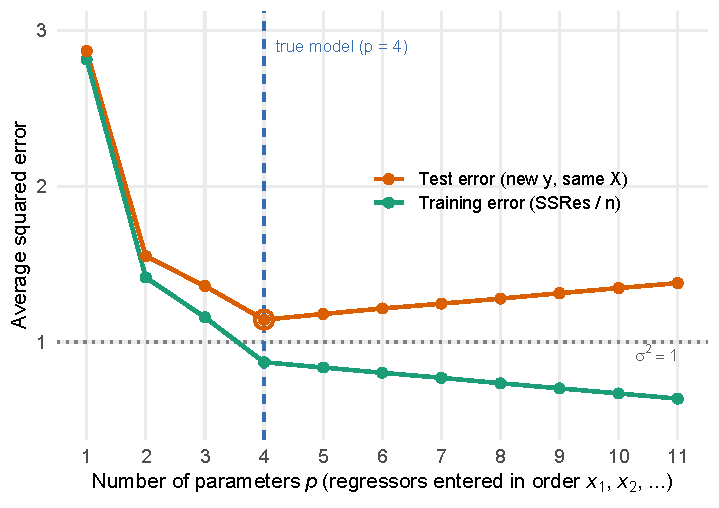
\includegraphics[width=\linewidth]{figures/train-test-error.pdf}}
            \mode<article>{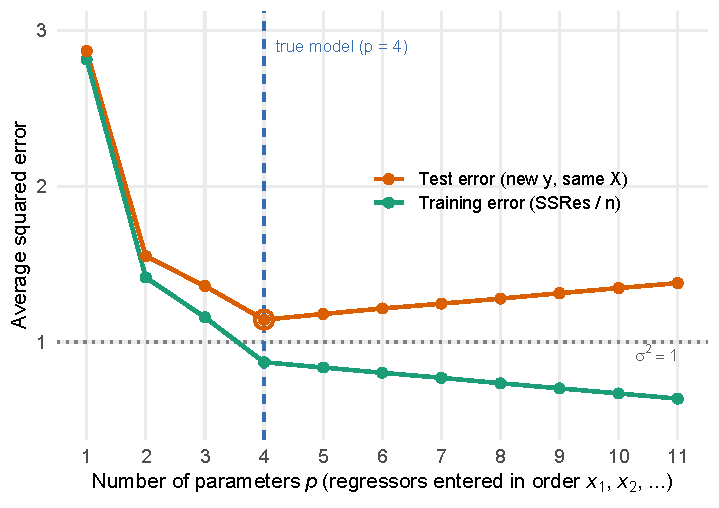
\includegraphics[width=0.75\linewidth]{figures/train-test-error.pdf}}
        \end{column}
    \end{columns}
\end{frame}


\begin{frame}{Grading Your Own Exam}
    The training error is too optimistic because the same data were used to fit the model and to grade it. For a model with no bias:
    \[
    \E[\SSRes(p)]=(n-p)\,\sigma^2,
    \qquad
    \E\Bigl[\textstyle\sum_i (y_i^{\text{new}}-\hat y_i)^2\Bigr]=(n+p)\,\sigma^2 .
    \]
    \begin{itemize}
        \item The fit chases the noise in its own data, so on its own data it looks $p\sigma^2$ better than the noise level. On new data it is $p\sigma^2$ worse: the cost of estimating $p$ parameters.
        \item The gap between the two is $2p\sigma^2$. Simulation at $p=4$: $\sigma^2(1-p/n)=0.867$ against 0.870, and $\sigma^2(1+p/n)=1.133$ against 1.14.
        \item Every criterion in this lecture adds a penalty to the training error to correct this optimism. They differ in how large the penalty is.
    \end{itemize}
\end{frame}


\begin{frame}{Question: Is Dropping a Real Effect Always Wrong?}
    \begin{itemize}
        \item Suppose the true coefficient of $x_4$ is not zero, but small. Dropping $x_4$ biases $\hat{\beta}_2$. Can the subset estimate still be \emph{better}?
        \item What does ``better'' have to mean for the answer to be yes?
    \end{itemize}
    % Answer:
    % - Yes, if better means smaller mean squared error: MSE = bias^2 + variance. Dropping x4 adds a small bias but removes a large variance (se of b2 0.186 -> 0.046).
    % - MPV 10.1.2: the subset estimate has smaller MSE whenever the dropped coefficients are small compared with their standard errors in the full model (roughly |beta_r| < se(beta_r_hat)).
    % - So "the true model" and "the best model to use" are different questions. This is why criteria that aim at prediction can leave out real but weak effects.
\end{frame}


\begin{frame}{How Many Candidate Models?}
    Every regressor is in or out, so there are $2^K$ subsets.
    \begin{center}
        \small
        \begin{tabular}{rr}
            \toprule
            $K$ & Subsets \\
            \midrule
            4 & 16 \\
            10 & 1\,024 \\
            20 & 1\,048\,576 \\
            40 & about $1.1\times10^{12}$ \\
            \bottomrule
        \end{tabular}
    \end{center}
    Two ways out:
    \begin{itemize}
        \item \textbf{Search} cleverly: add or remove one regressor at a time (sequential methods).
        \item \textbf{Score} every subset with a criterion and take the best (all possible regressions). Clever algorithms (``leaps and bounds'') make this feasible up to $K\approx30$--40.
    \end{itemize}
\end{frame}


\section{Sequential Selection}


\begin{frame}{The Engine: The Partial $F$-Test}
    From Lecture 9: adding one regressor $x_j$ to a model with $p$ parameters gives the partial $F$ statistic
    \[
    F_j=\frac{\SSR(\beta_j\mid\bbeta_p)}{\MSRes(\bbeta_p,\beta_j)}
    =\frac{\SSRes(p)-\SSRes(p+1)}{\SSRes(p+1)/(n-p-1)} = t_j^2 ,
    \]
    where $t_j$ is the $t$ statistic of $x_j$ in the larger model.
    \begin{itemize}
        \item Large $F_j$: $x_j$ explains a good share of what the current model leaves unexplained.
        \item The algorithms compare $F_j$ with a threshold: $F_{\text{IN}}$ to enter, $F_{\text{OUT}}$ to remove.
        \item We use $F_{\text{IN}}=F_{\text{OUT}}=4$, a common rule of thumb (close to a 5\% test when the residual df are moderate).
    \end{itemize}
\end{frame}


\subsection{Forward Selection}


\begin{frame}{Forward Selection}
    \begin{enumerate}
        \item Start with the intercept-only model.
        \item For each regressor not in the model, compute its partial $F$ for entering.
        \item If the largest of them exceeds $F_{\text{IN}}$, add that regressor; otherwise stop.
        \item Go back to step 2.
    \end{enumerate}
    \svspace{0.5em}
    \begin{itemize}
        \item The first regressor in is the one most correlated with $y$.
        \item After that, the next one in is the one with the largest \emph{partial} correlation with $y$: the one that best explains what is left after the regressors already in.
    \end{itemize}
\end{frame}


\begin{frame}{Forward Selection on the Cement Data}
    \begin{center}
        \small
        \begin{tabular}{clll}
            \toprule
            Step & In the model & Partial $F$ to enter & Action \\
            \midrule
            1 & (none) & $x_1$ 12.60, $x_2$ 21.96, $x_3$ 4.40, $x_4$ \textbf{22.80} & enter $x_4$ \\
            2 & $x_4$ & $x_1$ \textbf{108.22}, $x_2$ 0.17, $x_3$ 40.29 & enter $x_1$ \\
            3 & $x_4,x_1$ & $x_2$ \textbf{5.03}, $x_3$ 4.24 & enter $x_2$ \\
            4 & $x_4,x_1,x_2$ & $x_3$ 0.02 & stop \\
            \bottomrule
        \end{tabular}
    \end{center}
    \begin{itemize}
        \item Final model: $\{x_1,x_2,x_4\}$.
        \item At step 1, $x_2$ and $x_4$ are almost tied (21.96 and 22.80). At step 2, once $x_4$ is in, $x_2$ is worth almost nothing (0.17).
    \end{itemize}
\end{frame}


\begin{frame}{Question: Why Does $x_2$ Collapse After $x_4$ Enters?}
    \begin{itemize}
        \item On its own, $x_2$ is the second-best single predictor of heat. After $x_4$ enters, its partial $F$ drops from 21.96 to 0.17. Why?
        \item Forward selection then enters $x_2$ at step 3 anyway. What has changed by then?
    \end{itemize}
    % Answer:
    % - r(x2, x4) = -0.973: x2 is almost a copy of x4 (with the sign flipped). Once x4 is in, x2 carries almost no new information about y.
    % - After x1 is in, the small part of x2 that is not explained by x4 becomes useful (partial F 5.03). But now x4 is nearly redundant given x1 and x2, and forward selection has no way to take it out again.
\end{frame}


\subsection{Backward Elimination}


\begin{frame}{Backward Elimination}
    \begin{enumerate}
        \item Start with all $K$ regressors.
        \item For each regressor in the model, compute its partial $F$ as if it had entered last (equivalently, $t_j^2$).
        \item If the smallest of them is below $F_{\text{OUT}}$, remove that regressor; otherwise stop.
        \item Refit and go back to step 2.
    \end{enumerate}
    \svspace{0.5em}
    \begin{itemize}
        \item Every regressor gets judged in the presence of all the others: a good start when $K$ is moderate.
        \item Needs the full model to be estimable ($n>K+1$), and is unreliable when the full model suffers from strong multicollinearity, as here.
    \end{itemize}
\end{frame}


\begin{frame}{Backward Elimination on the Cement Data}
    \begin{center}
        \small
        \begin{tabular}{clll}
            \toprule
            Step & In the model & Partial $F$ of each regressor & Action \\
            \midrule
            1 & $x_1,x_2,x_3,x_4$ & $x_1$ 4.34, $x_2$ 0.50, $x_3$ \textbf{0.02}, $x_4$ 0.04 & remove $x_3$ \\
            2 & $x_1,x_2,x_4$ & $x_1$ 154.01, $x_2$ 5.03, $x_4$ \textbf{1.86} & remove $x_4$ \\
            3 & $x_1,x_2$ & $x_1$ 146.52, $x_2$ 208.58 & stop \\
            \bottomrule
        \end{tabular}
    \end{center}
    \begin{itemize}
        \item Final model: $\{x_1,x_2\}$. Not the same as forward selection.
        \item At step 1, every regressor except $x_1$ looks useless: the multicollinearity signature from Lecture 10. Each one can be imitated by the other three.
    \end{itemize}
\end{frame}


\subsection{Stepwise Regression}


\begin{frame}{Stepwise Regression}
    Forward selection that \emph{reconsiders}: after each entry, test every regressor already in the model for removal (Efroymson, 1960).
    \begin{center}
        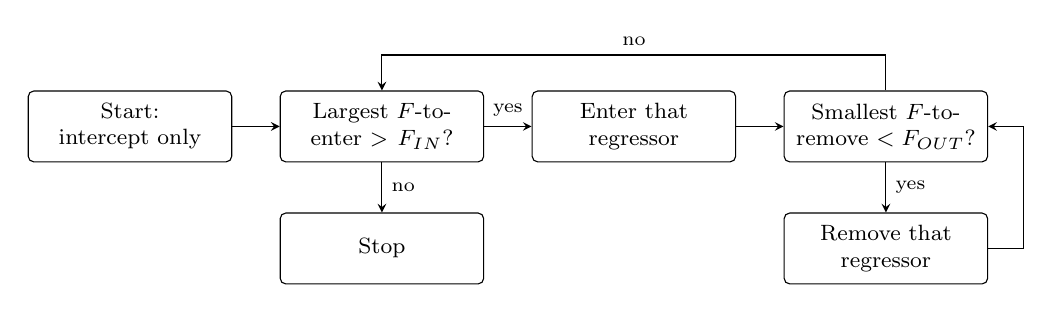
\begin{tikzpicture}[>=stealth, node distance=0.6cm and 0.55cm,
            box/.style={draw, rounded corners=2pt, align=center, font=\footnotesize, text width=2.35cm, minimum height=0.9cm, fill=white},
            lab/.style={font=\scriptsize}]
            \node[box] (start) at (0,0) {Start:\\ intercept only};
            \node[box] (q1) at (3.2,0) {Largest $F$-to-enter $>F_{\text{IN}}$?};
            \node[box] (add) at (6.4,0) {Enter that regressor};
            \node[box] (q2) at (9.6,0) {Smallest $F$-to-remove $<F_{\text{OUT}}$?};
            \node[box] (stop) at (3.2,-1.55) {Stop};
            \node[box] (rem) at (9.6,-1.55) {Remove that regressor};
            \draw[->] (start) -- (q1);
            \draw[->] (q1) -- node[lab, above] {yes} (add);
            \draw[->] (add) -- (q2);
            \draw[->] (q1) -- node[lab, right] {no} (stop);
            \draw[->] (q2) -- node[lab, right] {yes} (rem);
            \draw[->] (rem.east) -- ++(0.45,0) |- (q2.east);
            \draw[->] (q2.north) -- ++(0,0.45) -| node[lab, above, pos=0.25] {no} (q1.north);
        \end{tikzpicture}
    \end{center}
    \small
    \begin{itemize}
        \item A regressor that entered early can leave once others make it redundant.
        \item Choose $F_{\text{IN}}\ge F_{\text{OUT}}$; otherwise a regressor could enter and leave forever.
    \end{itemize}
\end{frame}


\begin{frame}{Stepwise Regression on the Cement Data}
    $F_{\text{IN}}=F_{\text{OUT}}=4$:
    \begin{enumerate}
        \item Enter $x_4$ ($F=22.80$).
        \item Enter $x_1$ ($F=108.22$). Check for removal: $x_4$ 159.30, $x_1$ 108.22. Both stay.
        \item Enter $x_2$ ($F=5.03$). Check for removal: $x_1$ 154.01, $x_2$ 5.03, $x_4$ \textbf{1.86}. \textbf{Remove $x_4$}.
        \item Candidates to enter: $x_3$ ($1.83$), $x_4$ ($1.86$). Neither passes 4. Stop.
    \end{enumerate}
    \svspace{0.3em}
    Final model: $\{x_1,x_2\}$, the same as backward elimination. The regressor that entered \emph{first} is the one that was thrown out.
\end{frame}


\begin{frame}{Three Algorithms, One Lattice of Models}
    \begin{columns}[T]
        \begin{column}{0.66\textwidth}
            \centering
            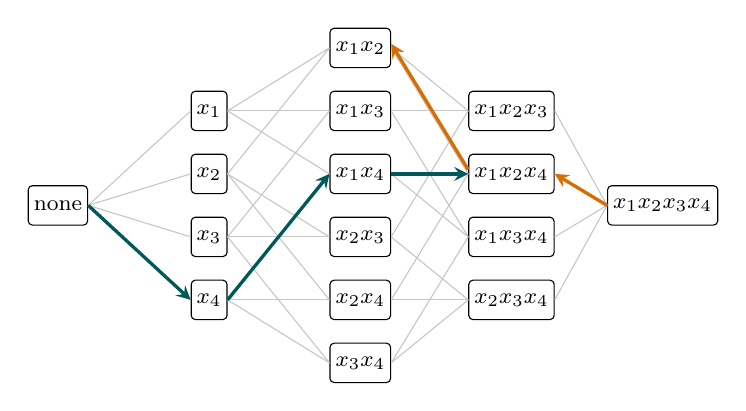
\begin{tikzpicture}[x=1.92cm, y=0.8cm, >=stealth,
                m/.style={draw, rounded corners=1.5pt, fill=white, font=\footnotesize, inner sep=2pt, minimum height=0.5cm},
                e/.style={gray!45, thin}]
                % models by size: column = number of regressors
                \node[m] (n0) at (0,0) {none};
                \node[m] (a1) at (1,1.5) {$x_1$};
                \node[m] (a2) at (1,0.5) {$x_2$};
                \node[m] (a3) at (1,-0.5) {$x_3$};
                \node[m] (a4) at (1,-1.5) {$x_4$};
                \node[m] (b12) at (2,2.5) {$x_1x_2$};
                \node[m] (b13) at (2,1.5) {$x_1x_3$};
                \node[m] (b14) at (2,0.5) {$x_1x_4$};
                \node[m] (b23) at (2,-0.5) {$x_2x_3$};
                \node[m] (b24) at (2,-1.5) {$x_2x_4$};
                \node[m] (b34) at (2,-2.5) {$x_3x_4$};
                \node[m] (c123) at (3,1.5) {$x_1x_2x_3$};
                \node[m] (c124) at (3,0.5) {$x_1x_2x_4$};
                \node[m] (c134) at (3,-0.5) {$x_1x_3x_4$};
                \node[m] (c234) at (3,-1.5) {$x_2x_3x_4$};
                \node[m] (d) at (4,0) {$x_1x_2x_3x_4$};
                % all one-step moves
                \foreach \s/\t in {n0/a1, n0/a2, n0/a3, n0/a4,
                    a1/b12, a1/b13, a1/b14, a2/b12, a2/b23, a2/b24, a3/b13, a3/b23, a3/b34, a4/b14, a4/b24, a4/b34,
                    b12/c123, b12/c124, b13/c123, b13/c134, b14/c124, b14/c134, b23/c123, b23/c234, b24/c124, b24/c234, b34/c134, b34/c234,
                    c123/d, c124/d, c134/d, c234/d}
                    \draw[e] (\s.east) -- (\t.west);
                % forward path (teal) and backward path (orange)
                \draw[->, very thick, teal!70!black] (n0.east) -- (a4.west);
                \draw[->, very thick, teal!70!black] (a4.east) -- (b14.west);
                \draw[->, very thick, teal!70!black] (b14.east) -- (c124.west);
                \draw[->, very thick, orange!85!black] (d.west) -- (c124.east);
                \draw[->, very thick, orange!85!black, transform canvas={yshift=1.5pt}] (c124.west) -- (b12.east);
            \end{tikzpicture}
        \end{column}
        \begin{column}{0.34\textwidth}
            \footnotesize
            \begin{itemize}
                \item Boxes: the 16 subsets. Lines: one regressor added or removed.
                \item \textcolor{teal!70!black}{\textbf{Forward}}: none $\to x_4\to x_1x_4\to x_1x_2x_4$.
                \item \textcolor{orange!85!black}{\textbf{Backward}}: full $\to x_1x_2x_4\to x_1x_2$.
                \item \textbf{Stepwise}: the forward path, then one step back.
                \item Each method sees only a few of the 16 models.
            \end{itemize}
        \end{column}
    \end{columns}
\end{frame}


\begin{frame}{The Threshold Matters}
    \begin{itemize}
        \item Forward selection with an exact 5\% test instead of 4: at step 3 the cutoff is $F_{0.05,1,9}=5.12$. $x_2$ has $F=5.03$ and does \emph{not} enter, so forward selection stops at $\{x_1,x_4\}$.
        \item Three reasonable procedures, three different final models: $\{x_1,x_2,x_4\}$, $\{x_1,x_2\}$, $\{x_1,x_4\}$.
    \end{itemize}
    \svspace{0.5em}
    \textbf{The nominal $\alpha$ is not the real $\alpha$.}
    \begin{itemize}
        \item At each step we test the \emph{largest} (or smallest) of several correlated $F$ statistics, so the usual $F$ distribution does not apply. Compare testing the largest of $n$ R-student values in Lecture 11.
        \item Treat $F_{\text{IN}}$ and $F_{\text{OUT}}$ as tuning knobs, not as significance levels.
    \end{itemize}
\end{frame}


\begin{frame}{Sequential Methods: Strengths and Weaknesses}
    \textbf{Strengths}
    \begin{itemize}
        \item Cheap: at most about $K^2/2$ fits instead of $2^K$. Usable with hundreds of candidates.
        \item Easy to explain, and available in every package.
    \end{itemize}
    \svspace{0.3em}
    \textbf{Weaknesses}
    \begin{itemize}
        \item One path through the lattice: no guarantee of finding the best subset of any size.
        \item Sensitive to the thresholds and to multicollinearity.
        \item They return \emph{one} model and hide close competitors.
    \end{itemize}
    \svspace{0.3em}
    Cement data so far: $\{x_1,x_2,x_4\}$ or $\{x_1,x_2\}$? To settle it we need a criterion that scores every model.
\end{frame}


\section{All Possible Regressions}


\subsection{Classical Criteria}


\begin{frame}{Fit Every Subset}
    With $K=4$ we can fit all 16 subsets. The best few, and the full model:
    \begin{center}
        \footnotesize
        \setlength{\tabcolsep}{5pt}
        \begin{tabular}{lcrrrrrr}
            \toprule
            Model & $p$ & $\SSRes$ & $R^2$ & $\Radj$ & $\MSRes$ & $C_p$ & $\PRESS$ \\
            \midrule
            $x_4$ & 2 & 883.87 & 0.6745 & 0.6450 & 80.35 & 138.73 & 1194.22 \\
            $x_1,x_2$ & 3 & 57.90 & 0.9787 & 0.9744 & 5.790 & \textbf{2.68} & 93.88 \\
            $x_1,x_4$ & 3 & 74.76 & 0.9725 & 0.9670 & 7.476 & 5.50 & 121.22 \\
            $x_1,x_2,x_3$ & 4 & 48.11 & 0.9823 & 0.9764 & 5.346 & 3.04 & 90.00 \\
            $x_1,x_2,x_4$ & 4 & 47.97 & 0.9823 & \textbf{0.9764} & \textbf{5.330} & 3.02 & \textbf{85.35} \\
            $x_1,x_3,x_4$ & 4 & 50.84 & 0.9813 & 0.9750 & 5.648 & 3.50 & 94.54 \\
            $x_1,x_2,x_3,x_4$ & 5 & 47.86 & 0.9824 & 0.9736 & 5.983 & 5.00 & 110.35 \\
            \bottomrule
        \end{tabular}
    \end{center}
    Bold: the best value of each criterion over all 16 subsets. The full table is in \texttt{figures/cement-allsubsets.csv}.
\end{frame}


\begin{frame}{$R^2$: Look for the Knee}
    \begin{itemize}
        \item $R^2$ never decreases when a regressor is added (Lecture 4), so maximizing it always picks the full model.
        \item Use it to see where adding regressors stops paying. Best $R^2$ of each size:
        \begin{center}
            \small
            \begin{tabular}{lcccc}
                \toprule
                $p$ & 2 & 3 & 4 & 5 \\
                \midrule
                Best subset & $x_4$ & $x_1,x_2$ & $x_1,x_2,x_4$ & all \\
                $R^2$ & 0.675 & 0.979 & 0.982 & 0.982 \\
                \bottomrule
            \end{tabular}
        \end{center}
        \item A huge jump from $p=2$ to $p=3$; after that, gains of at most $0.004$.
        \item $R^2$ shows the knee but cannot say which side of it to stop on.
    \end{itemize}
\end{frame}


\begin{frame}{Adjusted $R^2$ and $\MSRes$}
    \[
    \Radj=1-\frac{\MSRes(p)}{\SST/(n-1)}:
    \qquad \text{maximizing }\Radj\iff\text{minimizing }\MSRes(p).
    \]
    \begin{itemize}
        \item Cement data: both pick $\{x_1,x_2,x_4\}$ ($\MSRes=5.330$), a hair ahead of $\{x_1,x_2,x_3\}$ ($5.346$) and $\{x_1,x_2\}$ ($5.790$).
        \item Adding a regressor raises $\Radj$ whenever its partial $F$ exceeds \textbf{1}. That is a weak penalty: a useless regressor has partial $F>1$ about a third of the time.
        \item So $\Radj$ tends to choose models that are too large.
    \end{itemize}
\end{frame}


\begin{frame}{PRESS: Predict Each Point Without It}
    From Lecture 6: predict each $y_i$ from the model fitted \emph{without} observation $i$, and add up the squared errors:
    \[
    \PRESS_p=\sum_{i=1}^n\bigl(y_i-\hat y_{(i)}\bigr)^2=\sum_{i=1}^n\left(\frac{e_i}{1-h_{ii}}\right)^2 .
    \]
    \begin{itemize}
        \item No grading of your own exam: each point is graded by a model that never saw it. One fit is enough.
        \item Cement data: smallest for $\{x_1,x_2,x_4\}$ (85.35), then $\{x_1,x_2,x_3\}$ (90.00), $\{x_1,x_2\}$ (93.88); full model 110.35.
        \item Prediction $R^2$: $1-\PRESS/\SST=1-85.35/2715.76=0.969$ for $\{x_1,x_2,x_4\}$, and $0.965$ for $\{x_1,x_2\}$.
    \end{itemize}
\end{frame}


\begin{frame}{Best Subset of Each Size}
    \begin{center}
        % Figure: criteria-best-subset-cement.pdf (see selection-cement.R)
        \mode<presentation>{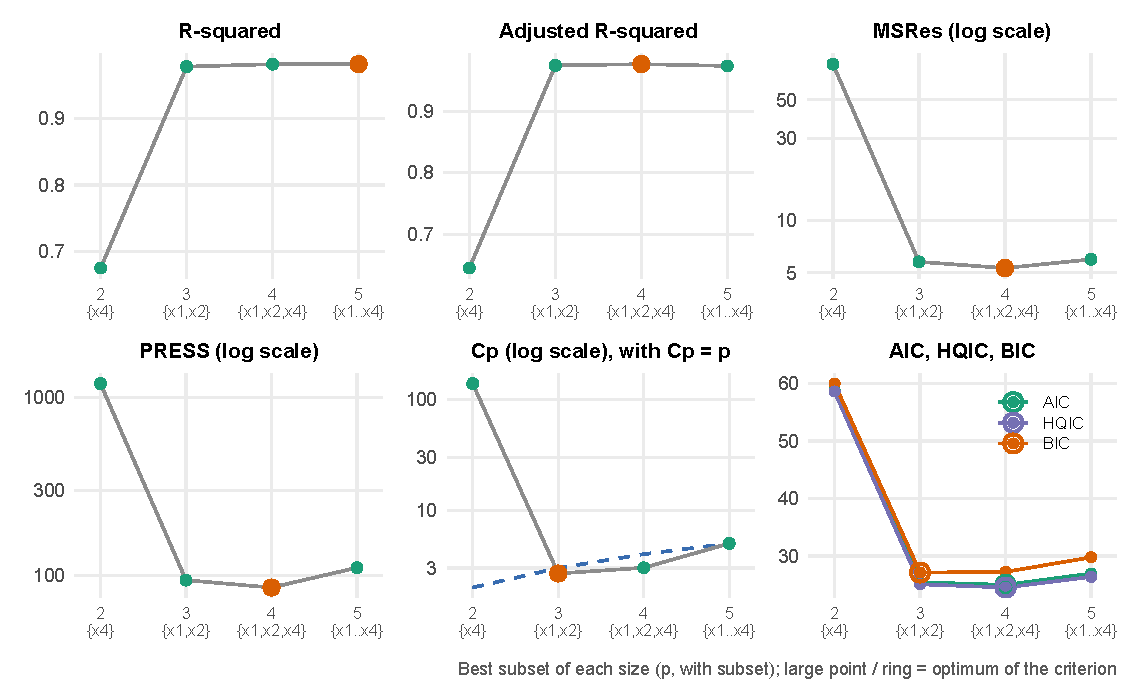
\includegraphics[height=0.72\textheight,width=\linewidth,keepaspectratio]{figures/criteria-best-subset-cement.pdf}}
        \mode<article>{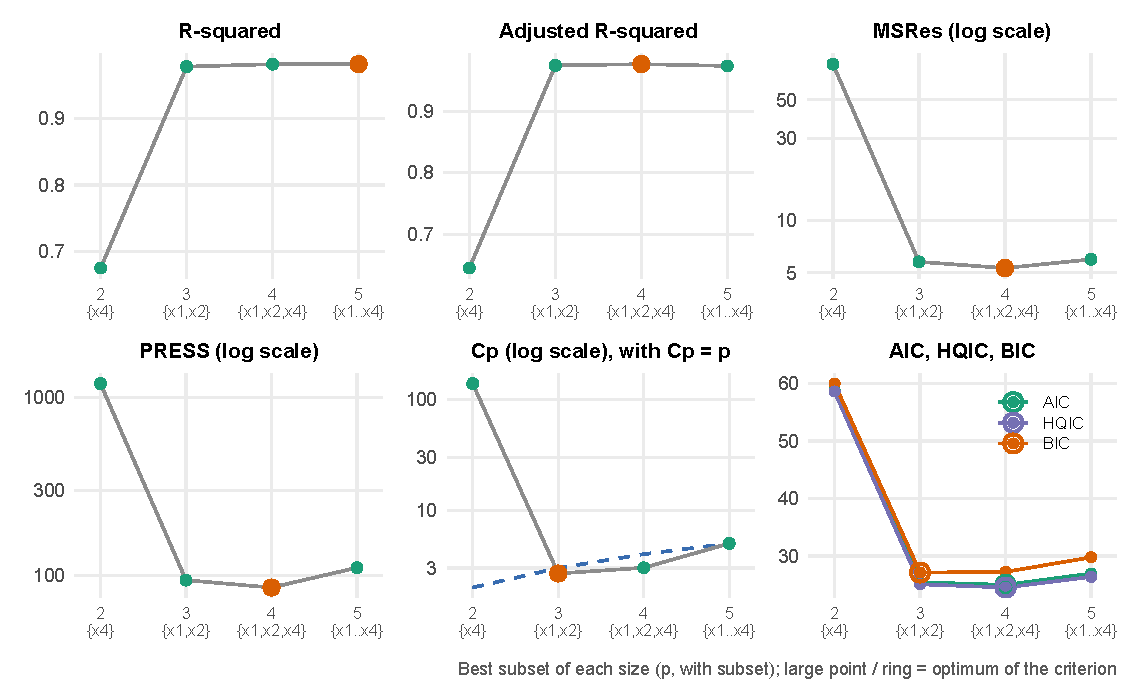
\includegraphics[width=\linewidth]{figures/criteria-best-subset-cement.pdf}}
    \end{center}
    \vspace{-0.5em}
    \footnotesize
    Every criterion agrees that $p=3$ is a huge improvement on $p=2$. They disagree about $p=3$ versus $p=4$.
\end{frame}


\subsection{Mallows' $C_p$}


\begin{frame}{What Should a Good Subset Minimize?}
    Mallows (1973): judge a subset by how far its fitted values are from the \emph{true} mean response, on average, in units of $\sigma^2$:
    \[
    \Gamma_p=\frac1{\sigma^2}\sum_{i=1}^n\E\bigl[\hat y_i-\E(y_i)\bigr]^2
    =\frac1{\sigma^2}\Biggl\{\underbrace{\sum_{i=1}^n\bigl[\E(\hat y_i)-\E(y_i)\bigr]^2}_{\text{bias}^2\ (\SSB)}
    +\underbrace{\sum_{i=1}^n\Var(\hat y_i)}_{\text{variance}}\Biggr\}.
    \]
    \begin{itemize}
        \item Too few regressors: the bias term is large.
        \item Too many: the variance term is large.
        \item $\Gamma_p$ is the total mean squared error of the fit. It depends on unknowns, so we have to estimate it.
    \end{itemize}
\end{frame}


\begin{frame}{Estimating the Two Parts}
    \textbf{Variance.} $\Var(\hat{\by})=\sigma^2\bH_p$, so
    \[
    \sum_{i=1}^n\Var(\hat y_i)=\sigma^2\tr(\bH_p)=p\,\sigma^2 ,
    \]
    the trace of the hat matrix again (Lecture 11): each parameter adds $\sigma^2$.
    \svspace{0.5em}
    \textbf{Bias.} The residual sum of squares absorbs the missing effects:
    \[
    \E[\SSRes(p)]=(n-p)\,\sigma^2+\SSB(p)
    \quad\Longrightarrow\quad
    \SSB(p)=\E[\SSRes(p)]-(n-p)\,\sigma^2 .
    \]
    Putting them together,
    \[
    \Gamma_p=\frac{\E[\SSRes(p)]}{\sigma^2}-n+2p .
    \]
\end{frame}


\begin{frame}{Mallows' $C_p$}
    Replace $\E[\SSRes(p)]$ by its observed value and $\sigma^2$ by $\hat\sigma^2=\MSRes$ of the \emph{full} model:
    \[
    C_p=\frac{\SSRes(p)}{\hat\sigma^2}-n+2p .
    \]
    \begin{itemize}
        \item If the subset has no bias, $\SSRes(p)\approx(n-p)\sigma^2$ and $C_p\approx p$. Subsets with bias lie \emph{above} the line $C_p=p$.
        \item For the full model, $C_{K+1}=K+1$ exactly. A useful check.
        \item Another way to read it: $\hat\sigma^2 C_p=\SSRes(p)+2p\hat\sigma^2-n\hat\sigma^2$, the training error plus a penalty of $2\hat\sigma^2$ per parameter. The penalty is the optimism $2p\sigma^2$ from the ``grading your own exam'' frame.
        \item Prefer subsets with small $C_p$, close to or below $p$.
    \end{itemize}
\end{frame}


\begin{frame}{Cement Data: The $C_p$ Plot}
    \begin{columns}[T]
        \begin{column}{0.40\textwidth}
            \footnotesize
            $\hat\sigma^2=5.983$ from the full model.
            \begin{itemize}
                \item $\{x_1,x_2\}$: $C_p=2.68<p=3$, the smallest of all.
                \item $p=4$: $\{x_1,x_2,x_4\}$ 3.02, $\{x_1,x_2,x_3\}$ 3.04, $\{x_1,x_3,x_4\}$ 3.50, all near the line.
                \item $\{x_1,x_4\}$: 5.50, above the line: bias.
                \item One-regressor models: $C_p>138$.
            \end{itemize}
            $C_p$ agrees with backward elimination and stepwise.
        \end{column}
        \begin{column}{0.60\textwidth}
            \centering
            % Figure: cp-plot-cement.pdf (see selection-cement.R)
            \mode<presentation>{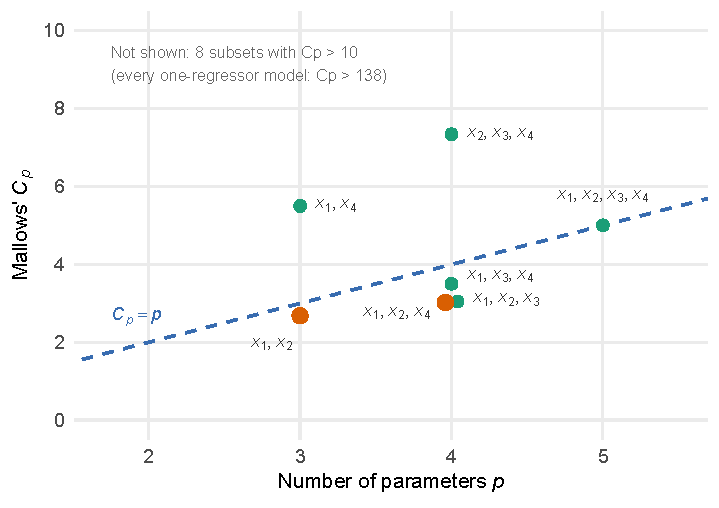
\includegraphics[width=\linewidth]{figures/cp-plot-cement.pdf}}
            \mode<article>{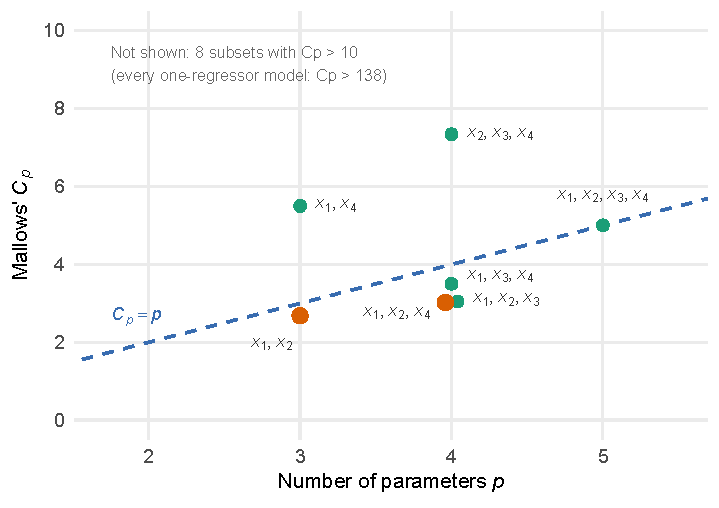
\includegraphics[width=0.75\linewidth]{figures/cp-plot-cement.pdf}}
        \end{column}
    \end{columns}
\end{frame}


\begin{frame}{Question: Below the Line}
    \begin{itemize}
        \item $\{x_1,x_2\}$ has $C_p=2.68$, below its $p=3$. Since $\Gamma_p\ge p$ for every subset (bias can only add), what does a value below $p$ mean?
        \item What would happen to every $C_p$ if the full model itself were badly wrong, say with a missing curvature term?
    \end{itemize}
    % Answer:
    % - Nothing special: C_p is an estimate of Gamma_p, and estimates scatter around their target. A value below p is consistent with no bias; it does not mean "better than unbiased".
    % - sigma^2-hat comes from the full model. If the full model is inadequate, sigma^2-hat is too large, every SSRes(p)/sigma^2-hat is too small, and all subsets look unbiased. C_p only compares subsets with the full model; it cannot detect what the full model is missing. Check the full model first (Lectures 6, 7, 10, 11).
\end{frame}


\section{Information Criteria}


\subsection{AIC}


\begin{frame}{From Least Squares to Likelihood}
    With normal errors, the maximized log-likelihood of a $p$-term model is (Lectures 3 and 4)
    \[
    -2\ln\hat L_p=n\ln(2\pi)+n\ln\!\left(\frac{\SSRes(p)}{n}\right)+n,
    \]
    using $\hat\sigma^2_{\ML}=\SSRes(p)/n$.
    \begin{itemize}
        \item Smaller $\SSRes$ means larger likelihood. So the maximized likelihood, like $R^2$, always favours the biggest model.
        \item The likelihood gives a common language for comparing models, also beyond least squares (logistic regression, time series, \dots).
        \item Information criteria add a penalty for the number of parameters.
    \end{itemize}
\end{frame}


\begin{frame}{Fit Plus Penalty}
    Every information criterion has the form
    \[
    \text{IC}=\underbrace{-2\ln\hat L}_{\text{lack of fit}}+\underbrace{c(n)\times k}_{\text{penalty}},
    \]
    with $k$ the number of estimated parameters. Smaller is better; only differences between models matter.
    \begin{center}
        \small
        \begin{tabular}{lll}
            \toprule
            Criterion & Penalty $c(n)$ & Aims at \\
            \midrule
            AIC & 2 & best prediction \\
            HQIC & $2\ln\ln n$ & the true model, with a light penalty \\
            BIC & $\ln n$ & the most probable model \\
            \bottomrule
        \end{tabular}
    \end{center}
\end{frame}


\begin{frame}{AIC: Correcting for Grading Your Own Exam}
    Akaike (1973): choose the model whose fitted distribution $\hat f$ is closest to the true distribution $g$ of the data, measured by the \emph{Kullback--Leibler divergence}
    \[
    \KL(g,\hat f)=\E_g\bigl[\ln g(Y)\bigr]-\E_g\bigl[\ln\hat f(Y)\bigr].
    \]
    \begin{itemize}
        \item The first term is the same for every model. So we want the model with the largest expected log-likelihood \emph{for new data}.
        \item $\ln\hat L$ on the data used for fitting is optimistic, just like $\SSRes$. Akaike showed that the optimism is about $k$, one unit per estimated parameter.
        \item Correcting for it:
        \[
        \AIC=-2\ln\hat L+2k .
        \]
    \end{itemize}
\end{frame}


\begin{frame}{AIC for Linear Regression}
    Dropping the terms that are the same for every model (MPV's form, also used by R's \texttt{step()} and \texttt{extractAIC()}):
    \[
    \AIC_p=n\ln\!\left(\frac{\SSRes(p)}{n}\right)+2p .
    \]
    \begin{itemize}
        \item R's \texttt{AIC()} keeps the constant $n\ln(2\pi)+n$ and counts $\sigma^2$ as a parameter ($k=p+1$): $+38.89$ for every cement model ($\{x_1,x_2\}$: $25.42$ or $64.31$). The ranking is the same.
        \item Small samples: AIC's penalty is too light when $n/k$ is small. The corrected version (Hurvich \& Tsai, 1989) is $\AICc=\AIC+2k(k+1)/(n-k-1)$, recommended when $n/k<40$. Cement data: $n/k\approx3$.
    \end{itemize}
\end{frame}


\subsection{BIC and HQIC}


\begin{frame}{BIC: Which Model Is Most Probable?}
    Schwarz (1978): give each model $M_j$ a prior probability and compute its posterior probability
    \[
    P(M_j\mid\by)\propto P(\by\mid M_j)\,P(M_j).
    \]
    \begin{itemize}
        \item $P(\by\mid M_j)$ averages the likelihood over the prior for the parameters. For large $n$,
        \[
        -2\ln P(\by\mid M_j)\approx-2\ln\hat L_j+k_j\ln n=\BIC_j .
        \]
        \item Regression form: $\BIC_p=n\ln(\SSRes(p)/n)+p\ln n$.
        \item With equal prior probabilities, $P(M_j\mid\by)\approx\exp(-\tfrac12\BIC_j)\big/\sum_m\exp(-\tfrac12\BIC_m)$.
        \item A BIC difference of 2 is odds of about $e\approx2.7$ to 1; a difference of 6, about 20 to 1.
    \end{itemize}
\end{frame}


\begin{frame}{HQIC}
    Hannan \& Quinn (1979):
    \[
    \HQIC_p=n\ln\!\left(\frac{\SSRes(p)}{n}\right)+2p\ln\ln n .
    \]
    \begin{itemize}
        \item Built from the law of the iterated logarithm: $2\ln\ln n$ is about the slowest-growing penalty that still picks the true model with probability tending to 1.
        \item A compromise between AIC (constant penalty) and BIC (penalty growing like $\ln n$).
        \item Popular in time series, for choosing the number of lags in autoregressive models.
    \end{itemize}
\end{frame}


\begin{frame}{Comparing the Penalties}
    \begin{columns}[T]
        \begin{column}{0.40\textwidth}
            \footnotesize
            \begin{itemize}
                \item BIC's penalty exceeds AIC's once $\ln n>2$, i.e.\ $n>e^2\approx7.4$. In practice: always.
                \item HQIC's exceeds AIC's only once $2\ln\ln n>2$, i.e.\ $n>e^e\approx15.2$.
                \item Cement data, $n=13$: AIC 2, \textbf{HQIC 1.88}, BIC 2.56. HQIC is the \emph{lightest} of the three here.
                \item At $n=1000$: AIC 2, HQIC 3.87, BIC 6.91.
            \end{itemize}
        \end{column}
        \begin{column}{0.60\textwidth}
            \centering
            % Figure: penalty-comparison.pdf (see selection-penalty.R)
            \mode<presentation>{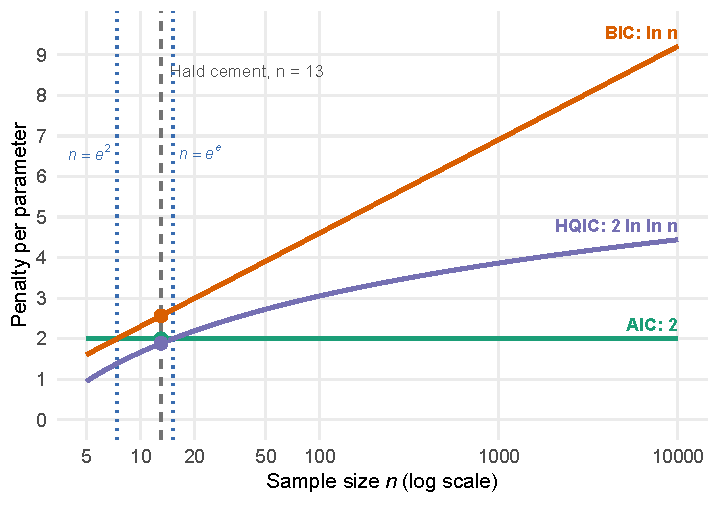
\includegraphics[width=\linewidth]{figures/penalty-comparison.pdf}}
            \mode<article>{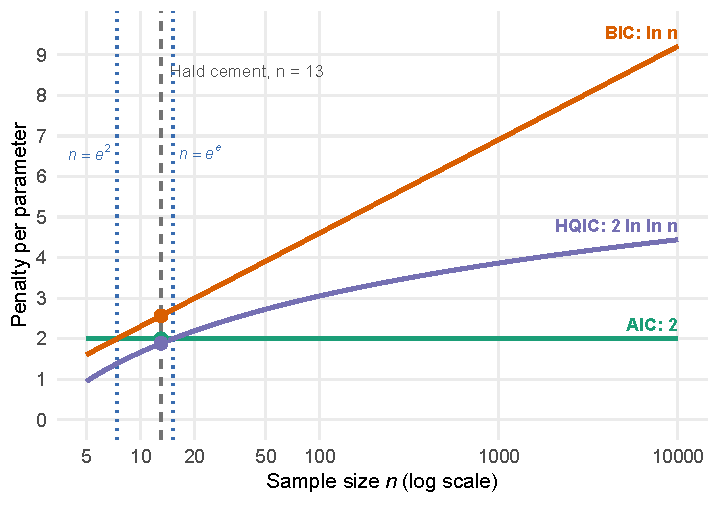
\includegraphics[width=0.75\linewidth]{figures/penalty-comparison.pdf}}
        \end{column}
    \end{columns}
\end{frame}


\begin{frame}{Consistent or Efficient?}
    \begin{itemize}
        \item \textbf{Consistent} (BIC, HQIC): if the true model is among the candidates, the probability of choosing it tends to 1 as $n\to\infty$.
        \item \textbf{Efficient} (AIC, $C_p$, PRESS): in large samples, the chosen model predicts as well as the best candidate, even if the true model is not among them. But the probability of including a useless regressor does not go to 0.
        \item Why AIC keeps overfitting: a useless regressor lowers AIC if its partial $F$ exceeds about 2, and in large samples that happens with probability $P(\chi^2_1>2)=0.157$, whatever $n$ is.
        \item No criterion has both properties (Yang, 2005).
    \end{itemize}
    \svspace{0.3em}
    Choose by purpose: \textbf{prediction $\to$ AIC-type}; \textbf{finding the structure $\to$ BIC-type}.
\end{frame}


\begin{frame}{Simulation: Finding the True Model}
    \vspace{-0.3em}
    \begin{center}
        % Figure: consistency-sim.pdf (see selection-simulation.R)
        \mode<presentation>{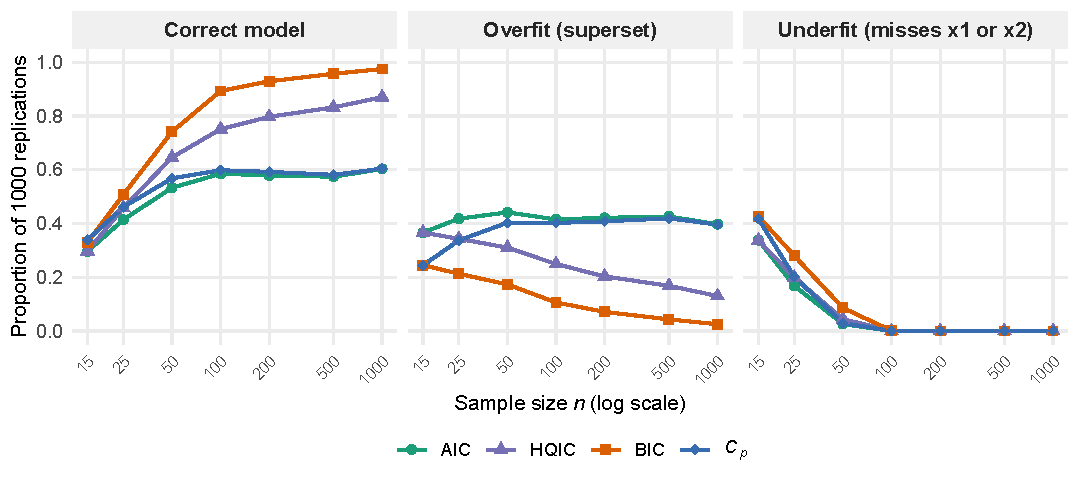
\includegraphics[height=0.5\textheight]{figures/consistency-sim.pdf}}
        \mode<article>{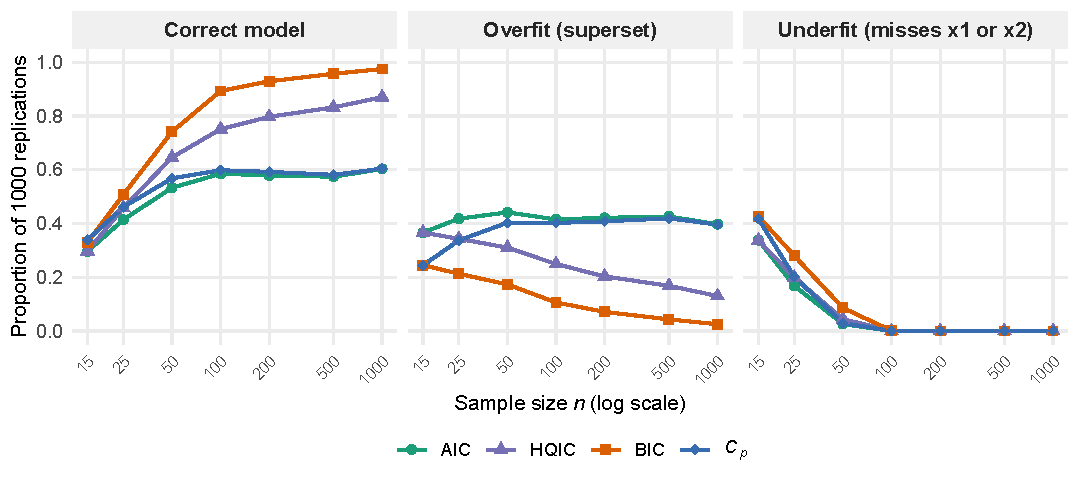
\includegraphics[width=\linewidth]{figures/consistency-sim.pdf}}
    \end{center}
    \vspace{-0.6em}
    \footnotesize
    5 candidates, true model $\{x_1,x_2\}$, all 32 subsets scored, 1000 replications per $n$.
    \begin{itemize}
        \item $n=1000$: BIC 0.98, HQIC 0.87, AIC and $C_p$ 0.60 $\approx(1-0.157)^3$ (each of 3 useless regressors gets in 16\% of the time).
        \item $n=15$: all near 0.3, and BIC \emph{underfits} most often (0.43). A heavy penalty also keeps out real effects.
    \end{itemize}
\end{frame}


\subsection{Cement Data}


\begin{frame}{Cement Data: AIC, HQIC and BIC}
    \begin{center}
        \small
        \begin{tabular}{lcrrrr}
            \toprule
            Model & $p$ & $\AIC$ & $\HQIC$ & $\BIC$ & $\AICc$ (R form) \\
            \midrule
            $x_1,x_2$ & 3 & 25.42 & 25.07 & \textbf{27.11} & \textbf{69.31} \\
            $x_1,x_4$ & 3 & 28.74 & 28.39 & 30.44 & 72.63 \\
            $x_1,x_2,x_3$ & 4 & 25.01 & 24.55 & 27.27 & 72.48 \\
            $x_1,x_2,x_4$ & 4 & \textbf{24.97} & \textbf{24.51} & 27.23 & 72.44 \\
            $x_1,x_3,x_4$ & 4 & 25.73 & 25.26 & 27.99 & 73.19 \\
            $x_1,x_2,x_3,x_4$ & 5 & 26.94 & 26.36 & 29.77 & 79.84 \\
            \bottomrule
        \end{tabular}
    \end{center}
    \begin{itemize}
        \item AIC and HQIC pick $\{x_1,x_2,x_4\}$. BIC and $\AICc$ pick $\{x_1,x_2\}$.
        \item On AIC the top three models are within 0.5 of each other.
    \end{itemize}
\end{frame}


\begin{frame}{How Close Is the Race?}
    \begin{columns}[T]
        \begin{column}{0.40\textwidth}
            \footnotesize
            $\Delta$ = criterion value minus the best value of that criterion.
            \begin{itemize}
                \item Burnham \& Anderson's rule of thumb: models with $\Delta<2$ have substantial support.
                \item Four or five subsets are inside that band, under all three criteria.
                \item What they share: $x_1$ and $x_2$, plus at most one of $x_3$, $x_4$.
                \item Given $x_1$ and $x_2$, adding $x_3$ is almost the same as adding $x_4$: the four percentages add up to about 100.
            \end{itemize}
        \end{column}
        \begin{column}{0.60\textwidth}
            \centering
            % Figure: ic-allsubsets-cement.pdf (see selection-cement.R)
            \mode<presentation>{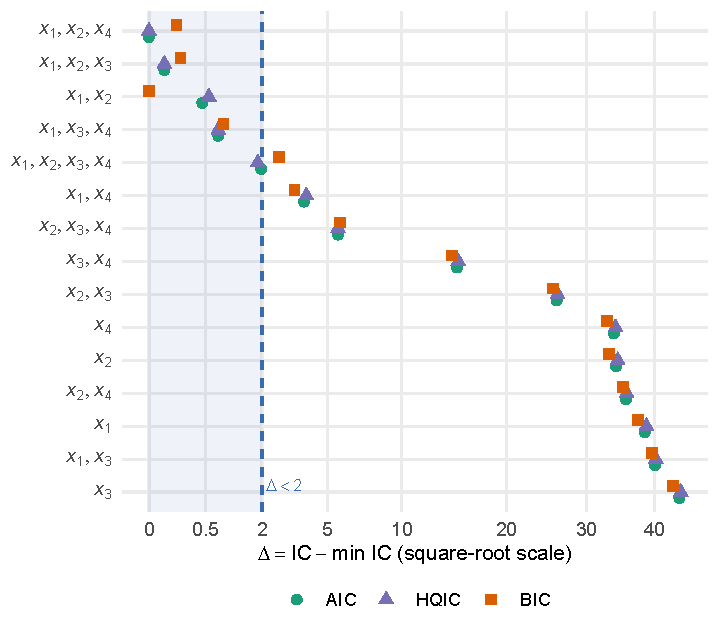
\includegraphics[height=0.8\textheight,width=\linewidth,keepaspectratio]{figures/ic-allsubsets-cement.pdf}}
            \mode<article>{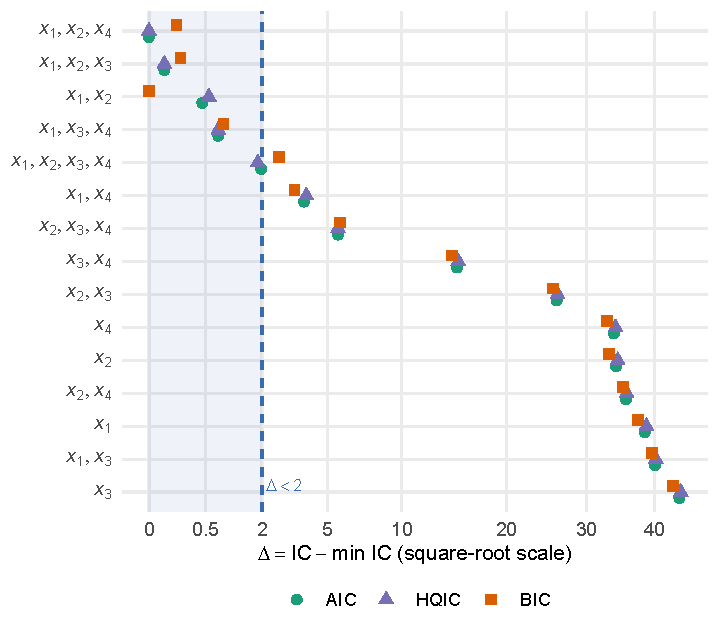
\includegraphics[width=0.7\linewidth]{figures/ic-allsubsets-cement.pdf}}
        \end{column}
    \end{columns}
\end{frame}


\begin{frame}{Model Weights}
    \begin{columns}[T]
        \begin{column}{0.45\textwidth}
            Turn criterion values into weights that add up to 1:
            \[
            w_j=\frac{\exp(-\tfrac12\Delta_j)}{\sum_m\exp(-\tfrac12\Delta_m)} .
            \]
            \begin{itemize}
                \item With AIC: \emph{Akaike weights}.
                \item With BIC: approximate posterior model probabilities.
            \end{itemize}
        \end{column}
        \begin{column}{0.55\textwidth}
            \centering
            \small
            \begin{tabular}{lrr}
                \toprule
                Model & Akaike & BIC \\
                & weight & probability \\
                \midrule
                $x_1,x_2,x_4$ & 0.247 & 0.234 \\
                $x_1,x_2,x_3$ & 0.242 & 0.230 \\
                $x_1,x_2$ & 0.197 & 0.248 \\
                $x_1,x_3,x_4$ & 0.169 & 0.161 \\
                $x_1,x_2,x_3,x_4$ & 0.092 & 0.066 \\
                \bottomrule
            \end{tabular}
        \end{column}
    \end{columns}
    \svspace{0.8em}
    No model gets more than a quarter of the support. Thirteen observations cannot tell these models apart.
\end{frame}


\begin{frame}{Every Criterion Is an Entry Fee}
    \small
    Adding one regressor to a $p$-term model lowers a criterion with penalty $c(n)$ per parameter exactly when its partial $F$ exceeds
    \[
    F^*=(n-p-1)\bigl(e^{c(n)/n}-1\bigr)\approx c(n)\quad\text{(large $n$)}.
    \]
    Cement data, adding $x_4$ to $\{x_1,x_2\}$ ($n-p-1=9$): \textbf{partial $F=1.86$}.
    \begin{center}
        \footnotesize
        \begin{tabular}{lrrrrrrr}
            \toprule
            & $\Radj$ & HQIC & AIC & BIC & $C_p$ & Stepwise & 5\% test \\
            \midrule
            Fee $F^*$ & 1.00 & 1.40 & 1.50 & 1.96 & 2.25 & 4.00 & 5.12 \\
            Keep $x_4$? & yes & yes & yes & no & no & no & no \\
            \bottomrule
        \end{tabular}
    \end{center}
    \begin{itemize}
        \item The whole disagreement is about one number: $x_4$ offers 1.86, and the fees range from 1 to 5.12.
        \item $x_3$ in place of $x_4$ offers 1.83 (given $x_1,x_2$ it carries nearly the same information, as the percentages sum to about 100): hence the three-way tie.
    \end{itemize}
    % C_p's fee is 2 sigma^2-hat / MSRes(p+1) = 2(5.983)/5.330 = 2.25, because it measures sigma^2 with the full model.
\end{frame}


\begin{frame}{Automatic Search with \texttt{step()}}
    R's \texttt{step()} does stepwise selection with an information criterion instead of $F$ thresholds: at each step it makes the single addition or removal that lowers the criterion most.
    \svspace{0.3em}
    \begin{itemize}
        \item \texttt{step(lm(y \textasciitilde{} 1, cement), scope = \textasciitilde{} x1 + x2 + x3 + x4)}, AIC ($k=2$): enters $x_4$, $x_1$, $x_2$ and stops at $\{x_1,x_2,x_4\}$ (AIC 24.97).
        \item Backward from the full model, AIC: also $\{x_1,x_2,x_4\}$.
        \item The same search with \texttt{k = log(13)}, i.e.\ BIC: $\{x_1,x_2\}$.
    \end{itemize}
    \svspace{0.3em}
    The search method matters less than the criterion. AIC-based stepwise is stepwise selection with an entry fee near 2 instead of 4.
\end{frame}


\begin{frame}{Question: Why Not Always Use the Heaviest Penalty?}
    \begin{itemize}
        \item BIC finds the true model more often in large samples. Why would anyone use AIC?
        \item For the cement data, which criterion would you trust if the goal were to predict the heat of a new batch? To decide which compounds affect the heat?
    \end{itemize}
    % Answer:
    % - A heavy penalty also keeps out real but weak effects, especially in small samples (BIC underfits 43% of the time at n = 15 in the simulation). Leaving out a real effect biases everything else.
    % - "The true model is among the candidates" is a strong assumption. If it is not (and in practice it rarely is), the consistency of BIC is about the closest candidate, while AIC aims directly at good prediction.
    % - Prediction: AIC/PRESS point to {x1,x2,x4}, but the differences are tiny (PRESS 85.35 vs 93.88). Explanation: the extra regressor in {x1,x2,x4} has a coefficient that cannot be estimated reliably; {x1,x2} is the honest structural summary.
\end{frame}


\section{Deviance Information Criterion}


\begin{frame}{A Minimal Bayesian Set-up}
    In Bayesian statistics the parameters are random: we start with a \emph{prior} $\pi(\btheta)$ and update it with the data to a \emph{posterior}
    \[
    \pi(\btheta\mid\by)\propto L(\btheta)\,\pi(\btheta).
    \]
    \begin{itemize}
        \item Regression with the reference prior $\pi(\bbeta,\sigma^2)\propto1/\sigma^2$ (no prior information): the posterior is known exactly.
        \[
        \sigma^2\mid\by\sim\frac{\SSRes}{\chi^2_{n-p}},
        \qquad
        \bbeta\mid\sigma^2,\by\sim N\bigl(\hat{\bbeta},\ \sigma^2(\bX'\bX)^{-1}\bigr).
        \]
        \item So we can simulate draws of $(\bbeta,\sigma^2)$ directly. For more complex models the draws come from Markov chain Monte Carlo (MCMC).
        \item Instead of one estimate we get thousands of plausible parameter values, and can ask how well the model fits across all of them.
    \end{itemize}
\end{frame}


\begin{frame}{DIC}
    Spiegelhalter et al.\ (2002). Deviance $D(\btheta)=-2\ln L(\btheta)$, computed for every posterior draw.
    \begin{columns}[T]
        \begin{column}{0.46\textwidth}
            \small
            \begin{itemize}
                \item \textbf{Fit}: posterior mean deviance $\bar D=\E[D(\btheta)\mid\by]$.
                \item \textbf{Complexity}: $p_D=\bar D-D(\bar{\btheta})$, with $\bar{\btheta}$ the posterior mean.
                \item $\DIC=\bar D+p_D$.
            \end{itemize}
            Same shape as AIC, but the parameter count $p_D$ is \emph{estimated} from the posterior.
        \end{column}
        \begin{column}{0.54\textwidth}
            \centering
            % Figure: deviance-posterior-cement.pdf (see dic-cement.R)
            \mode<presentation>{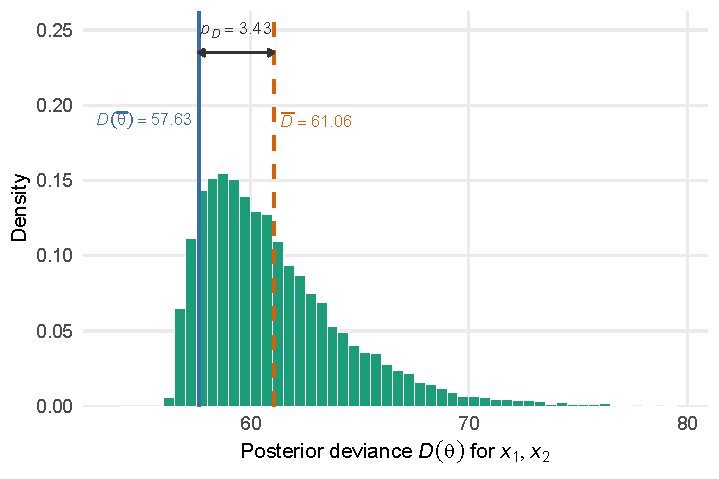
\includegraphics[width=\linewidth]{figures/deviance-posterior-cement.pdf}}
            \mode<article>{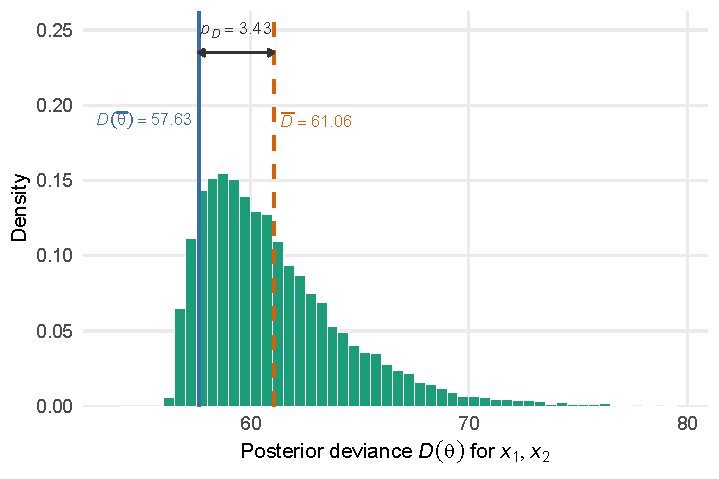
\includegraphics[width=0.7\linewidth]{figures/deviance-posterior-cement.pdf}}
            \par{\footnotesize $\{x_1,x_2\}$, 20\,000 posterior draws}
        \end{column}
    \end{columns}
\end{frame}


\begin{frame}{Cement Data: DIC}
    Flat prior, 20\,000 exact posterior draws per model.
    \begin{center}
        \small
        \begin{tabular}{lcrrrr}
            \toprule
            Model & $k$ & $\bar D$ & $p_D$ & DIC & AIC \\
            \midrule
            $x_1,x_2$ & 4 & 61.06 & 3.43 & 64.49 & 64.31 \\
            $x_1,x_4$ & 4 & 64.41 & 3.44 & 67.85 & 67.63 \\
            $x_1,x_2,x_3$ & 5 & 60.17 & 4.24 & 64.40 & 63.90 \\
            $x_1,x_2,x_4$ & 5 & 60.16 & 4.24 & 64.40 & 63.87 \\
            $x_1,x_3,x_4$ & 5 & 60.88 & 4.17 & 65.05 & 64.62 \\
            $x_1,x_2,x_3,x_4$ & 6 & 61.84 & 4.94 & 66.78 & 65.84 \\
            \bottomrule
        \end{tabular}
    \end{center}
    \begin{itemize}
        \item $k=p+1$ counts $\sigma^2$; AIC is in R's form, on the same scale as DIC.
        \item $p_D$ is close to $k$ (a little below, because $\sigma^2$ is plugged in at its posterior mean).
        \item The top three models are tied within simulation error.
    \end{itemize}
\end{frame}


\begin{frame}{DIC Against AIC}
    \begin{center}
        % Figure: dic-vs-aic-cement.pdf (see dic-cement.R)
        \mode<presentation>{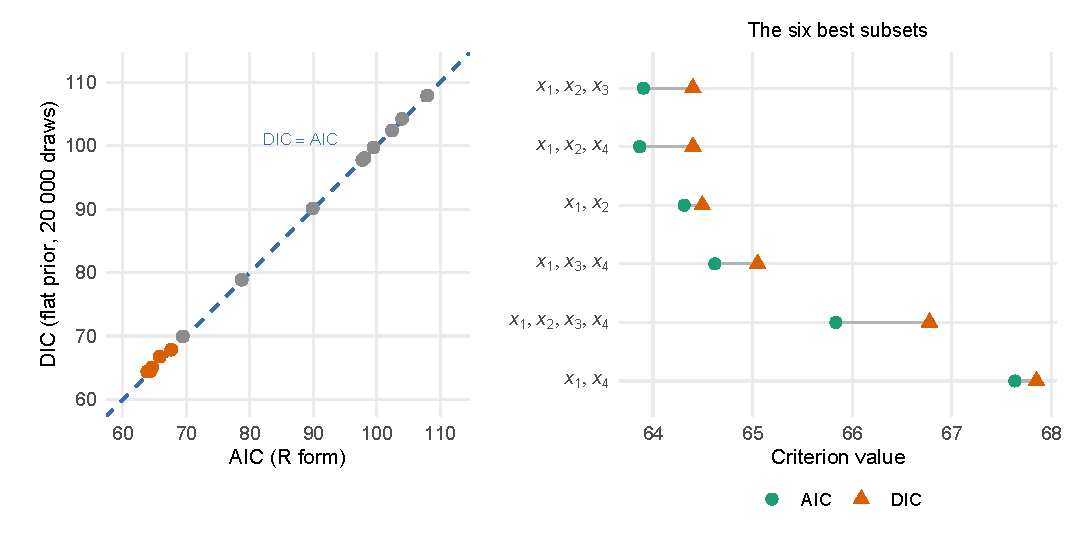
\includegraphics[width=0.92\linewidth,height=0.62\textheight,keepaspectratio]{figures/dic-vs-aic-cement.pdf}}
        \mode<article>{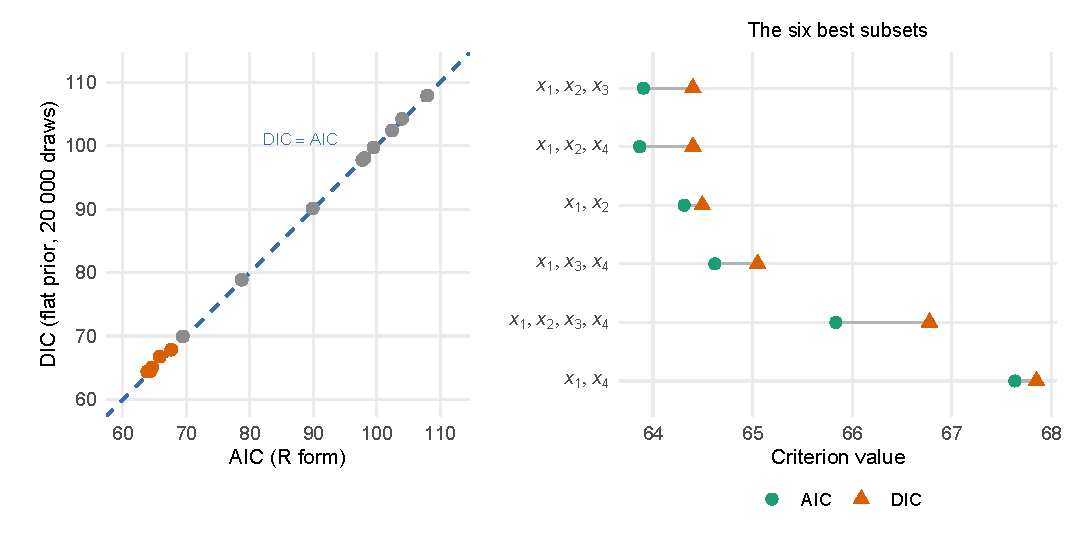
\includegraphics[width=0.9\linewidth]{figures/dic-vs-aic-cement.pdf}}
    \end{center}
    \vspace{-0.4em}
    With a flat prior, DIC and AIC agree to within 1 unit for all 15 subsets: DIC adds nothing new here. It earns its keep in models where AIC's parameter count is unclear.
\end{frame}


\begin{frame}{When Is DIC Useful?}
    \begin{itemize}
        \item With a flat prior and a simple model, DIC tells us nothing AIC does not. Its use is in models where ``the number of parameters'' is unclear:
        \begin{itemize}
            \item hierarchical (random-effects) models, where many parameters are pulled towards a common mean and each counts as less than one;
            \item models with informative priors, which also restrict the parameters.
        \end{itemize}
        In those models $p_D$ comes out smaller than the nominal count.
        \item DIC is computed directly from MCMC output, so it is built into Bayesian software.
        \item Limitations: it changes if the model is reparameterized, $p_D$ can even be negative, and it behaves poorly for mixture models. Newer alternatives: WAIC and leave-one-out cross-validation.
    \end{itemize}
\end{frame}


\section{Choosing a Model for the Cement Data}


\begin{frame}{The Verdict}
    \begin{center}
        \small
        \begin{tabular}{ll}
            \toprule
            Method or criterion & Selected model \\
            \midrule
            Forward selection ($F_{\text{IN}}=4$) & $\{x_1,x_2,x_4\}$ \\
            Forward selection (exact 5\% test) & $\{x_1,x_4\}$ \\
            Backward elimination, stepwise ($F=4$) & $\{x_1,x_2\}$ \\
            Max $\Radj$, min $\MSRes$, min $\PRESS$ & $\{x_1,x_2,x_4\}$ \\
            Min $C_p$ & $\{x_1,x_2\}$ \\
            Min AIC, HQIC & $\{x_1,x_2,x_4\}$, then $\{x_1,x_2,x_3\}$ \\
            Min BIC, $\AICc$ & $\{x_1,x_2\}$ \\
            Min DIC & three-way tie \\
            \bottomrule
        \end{tabular}
    \end{center}
    Every method includes $x_1$ and one of the near-copies $x_2$, $x_4$. They disagree about whether to add a second one.
\end{frame}


\begin{frame}{Why They Split: Collinearity Again}
    \begin{center}
        \small
        \begin{tabular}{lcc}
            \toprule
            & $\{x_1,x_2\}$ & $\{x_1,x_2,x_4\}$ \\
            \midrule
            Intercept & 52.58 (2.29) & 71.65 (14.14) \\
            $x_1$ & 1.468 (0.121) & 1.452 (0.117) \\
            $x_2$ & 0.662 (0.046) & 0.416 (0.186) \\
            $x_4$ & & $-0.237$ (0.173) \\
            \midrule
            VIFs & 1.06, 1.06 & 1.07, 18.78, 18.94 \\
            $\SSRes$, $\MSRes$ & 57.90, 5.79 & 47.97, 5.33 \\
            \bottomrule
        \end{tabular}
    \end{center}
    \begin{itemize}
        \item Adding $x_4$ lowers $\SSRes$ by 9.9, a little better than an average useless regressor would, at the price of an unstable pair of coefficients ($x_2$: $p=0.052$; $x_4$: $p=0.205$).
        \item Light penalties accept that trade; heavy penalties refuse it.
    \end{itemize}
\end{frame}


\begin{frame}{A Recommendation}
    \begin{itemize}
        \item \textbf{For explanation}: $\hat y=52.58+1.468\,x_1+0.662\,x_2$. Both coefficients are estimated precisely ($|t|>12$), the VIFs are 1.06, and $C_p$, BIC, $\AICc$, backward elimination and stepwise all choose it.
        \item \textbf{For prediction} within the range of the data, $\{x_1,x_2,x_4\}$ is marginally better ($\PRESS$ 85.35 against 93.88), but $x_2$ and $x_4$ move together in every sample, so the two models give almost the same predictions.
        \item \textbf{Report the shortlist}, not only the winner: $\{x_1,x_2\}$, $\{x_1,x_2,x_4\}$, $\{x_1,x_2,x_3\}$ are practically tied. A different sample of 13 cements could easily reverse their order.
        \item Then check the chosen model as any other: residuals (Lecture 6), influence (Lecture 11).
    \end{itemize}
\end{frame}


\begin{frame}{Inference After Selection}
    The $t$-tests, confidence intervals and $R^2$ printed for the selected model pretend that the model was fixed in advance. It was not: the same data chose it.
    \begin{itemize}
        \item The regressors that survive are the ones whose estimates happened to come out large: their coefficients are biased away from zero, and their $p$-values are too small (the \emph{winner's curse}).
        \item The standard errors ignore the uncertainty about which model is right.
    \end{itemize}
    \svspace{0.3em}
    How bad can it get? Freedman (1983) selected regressors from pure noise.
\end{frame}


\begin{frame}{Freedman's Paradox}
    \begin{columns}[T]
        \begin{column}{0.42\textwidth}
            \footnotesize
            $n=100$; $y$ and 50 regressors are independent noise: every true coefficient is 0.
            \begin{enumerate}
                \item Fit all 50; keep those with $p<0.25$.
                \item Refit with those; read the output as usual.
            \end{enumerate}
            Over 1000 replications: 12.3 regressors kept, 5.5 of them ``significant'' at 5\% (2.5 expected without selection), overall $F$ significant in 94\% of runs, average $R^2=0.31$.
        \end{column}
        \begin{column}{0.58\textwidth}
            \centering
            % Figure: freedman-paradox.pdf (see selection-simulation.R)
            \mode<presentation>{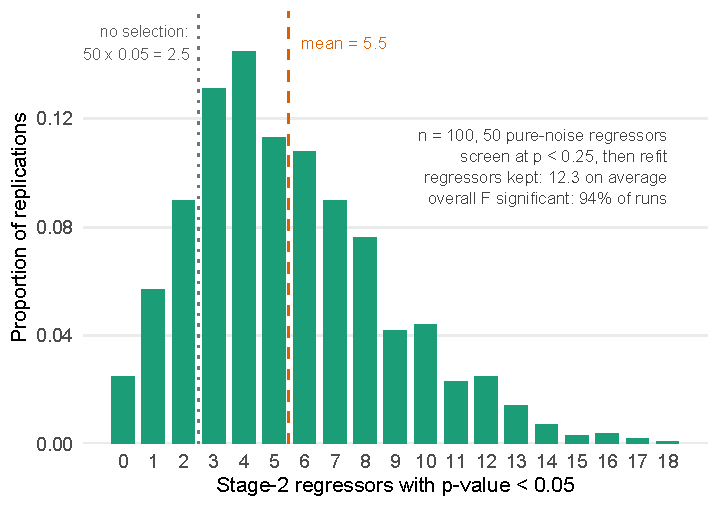
\includegraphics[width=\linewidth]{figures/freedman-paradox.pdf}}
            \mode<article>{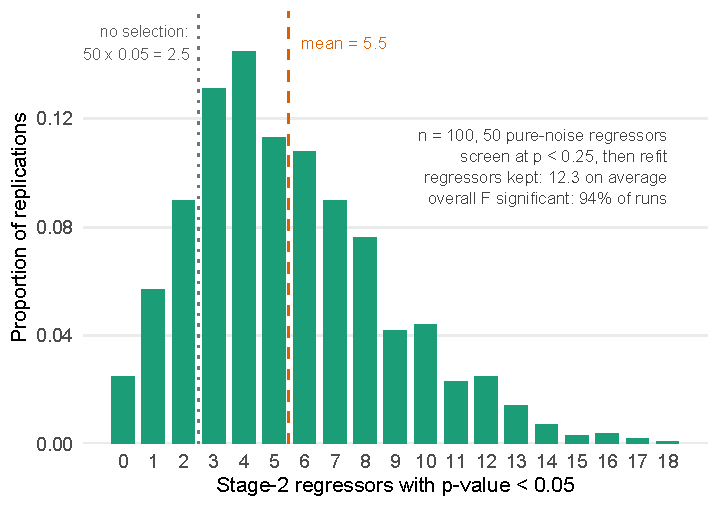
\includegraphics[width=0.75\linewidth]{figures/freedman-paradox.pdf}}
        \end{column}
    \end{columns}
\end{frame}


\begin{frame}{Question: Honest Inference After Selection}
    \begin{itemize}
        \item In Freedman's experiment, what single change to the procedure would make the stage-2 $p$-values honest again?
        \item Stepwise regression on the cement data reports $p<10^{-8}$ for both $x_1$ and $x_2$. Should that worry us as much?
    \end{itemize}
    % Answer:
    % - Use different data for choosing and for testing: split the sample, select on one half, fit and test on the other. Then the selection cannot have tuned itself to the noise in the test half. (Cost: fewer observations for each step.)
    % - Much less. The bias of post-selection p-values matters most for effects near the threshold. t = 12 and 14 are so far beyond any threshold that selection could not have manufactured them; x2 vs x4 (t = 2.2 and -1.4) is where the reported p-values cannot be taken at face value.
\end{frame}


\begin{frame}{A Model-Building Strategy}
    \begin{enumerate}
        \item \textbf{Fix the full model first.} Check residuals (Lecture 6), transformations (Lecture 7), multicollinearity (Lecture 10) and influence (Lecture 11). Selection on a broken full model selects from broken models.
        \item \textbf{Search.} All possible regressions when $K$ is moderate; otherwise stepwise as a screening device, run both forward and backward.
        \item \textbf{Shortlist} the models that are close on two or three criteria ($C_p$, AIC, BIC), instead of taking a single winner.
        \item \textbf{Re-check} the shortlisted models' diagnostics, and prefer the one that makes subject-matter sense.
        \item \textbf{Validate}: $\PRESS$, a hold-out sample, or new data. Be honest that the reported $p$-values come after selection.
    \end{enumerate}
\end{frame}


\section{Summary}


\begin{frame}{Selection Criteria at a Glance}
    \begin{center}
        \footnotesize
        \setlength{\tabcolsep}{4pt}
        \begin{tabular}{llll}
            \toprule
            Criterion & Formula & Fee ($F$) & Aims at \\
            \midrule
            $\Radj$, $\MSRes$ & $\SSRes/(n-p)$ & 1 & fit (weak penalty) \\
            $\PRESS$ & $\sum[e_i/(1-h_{ii})]^2$ & --- & prediction \\
            $C_p$ & $\SSRes/\hat\sigma^2-n+2p$ & $\approx2$ & prediction \\
            AIC & $n\ln(\SSRes/n)+2p$ & $\approx2$ & prediction \\
            HQIC & $n\ln(\SSRes/n)+2p\ln\ln n$ & $\approx2\ln\ln n$ & true model \\
            BIC & $n\ln(\SSRes/n)+p\ln n$ & $\approx\ln n$ & true model \\
            DIC & $\bar D+p_D$ & $\approx2$ (flat prior) & Bayesian models \\
            \bottomrule
        \end{tabular}
    \end{center}
    Smaller is better for all except $\Radj$. Sequential methods (forward, backward, stepwise) search with an $F$ fee, usually 4.
\end{frame}


\begin{frame}{Key Takeaways}
    \begin{itemize}
        \item Leaving out a regressor that matters causes bias; keeping one that does not costs variance. The best model to use need not be the true model.
        \item Forward selection, backward elimination and stepwise regression each walk one path through the $2^K$ models and can end in different places.
        \item Every criterion is training error plus a penalty for grading your own exam. They differ in the fee per parameter: about 2 for $C_p$ and AIC, $\ln n$ for BIC.
        \item AIC-type criteria aim at prediction and keep some useless regressors; BIC aims at the true model and can underfit in small samples.
        \item When models are close, report the shortlist, check diagnostics, and remember that $p$-values after selection are too optimistic.
    \end{itemize}
\end{frame}
